\begin{figure}[h!]
\begin{center}
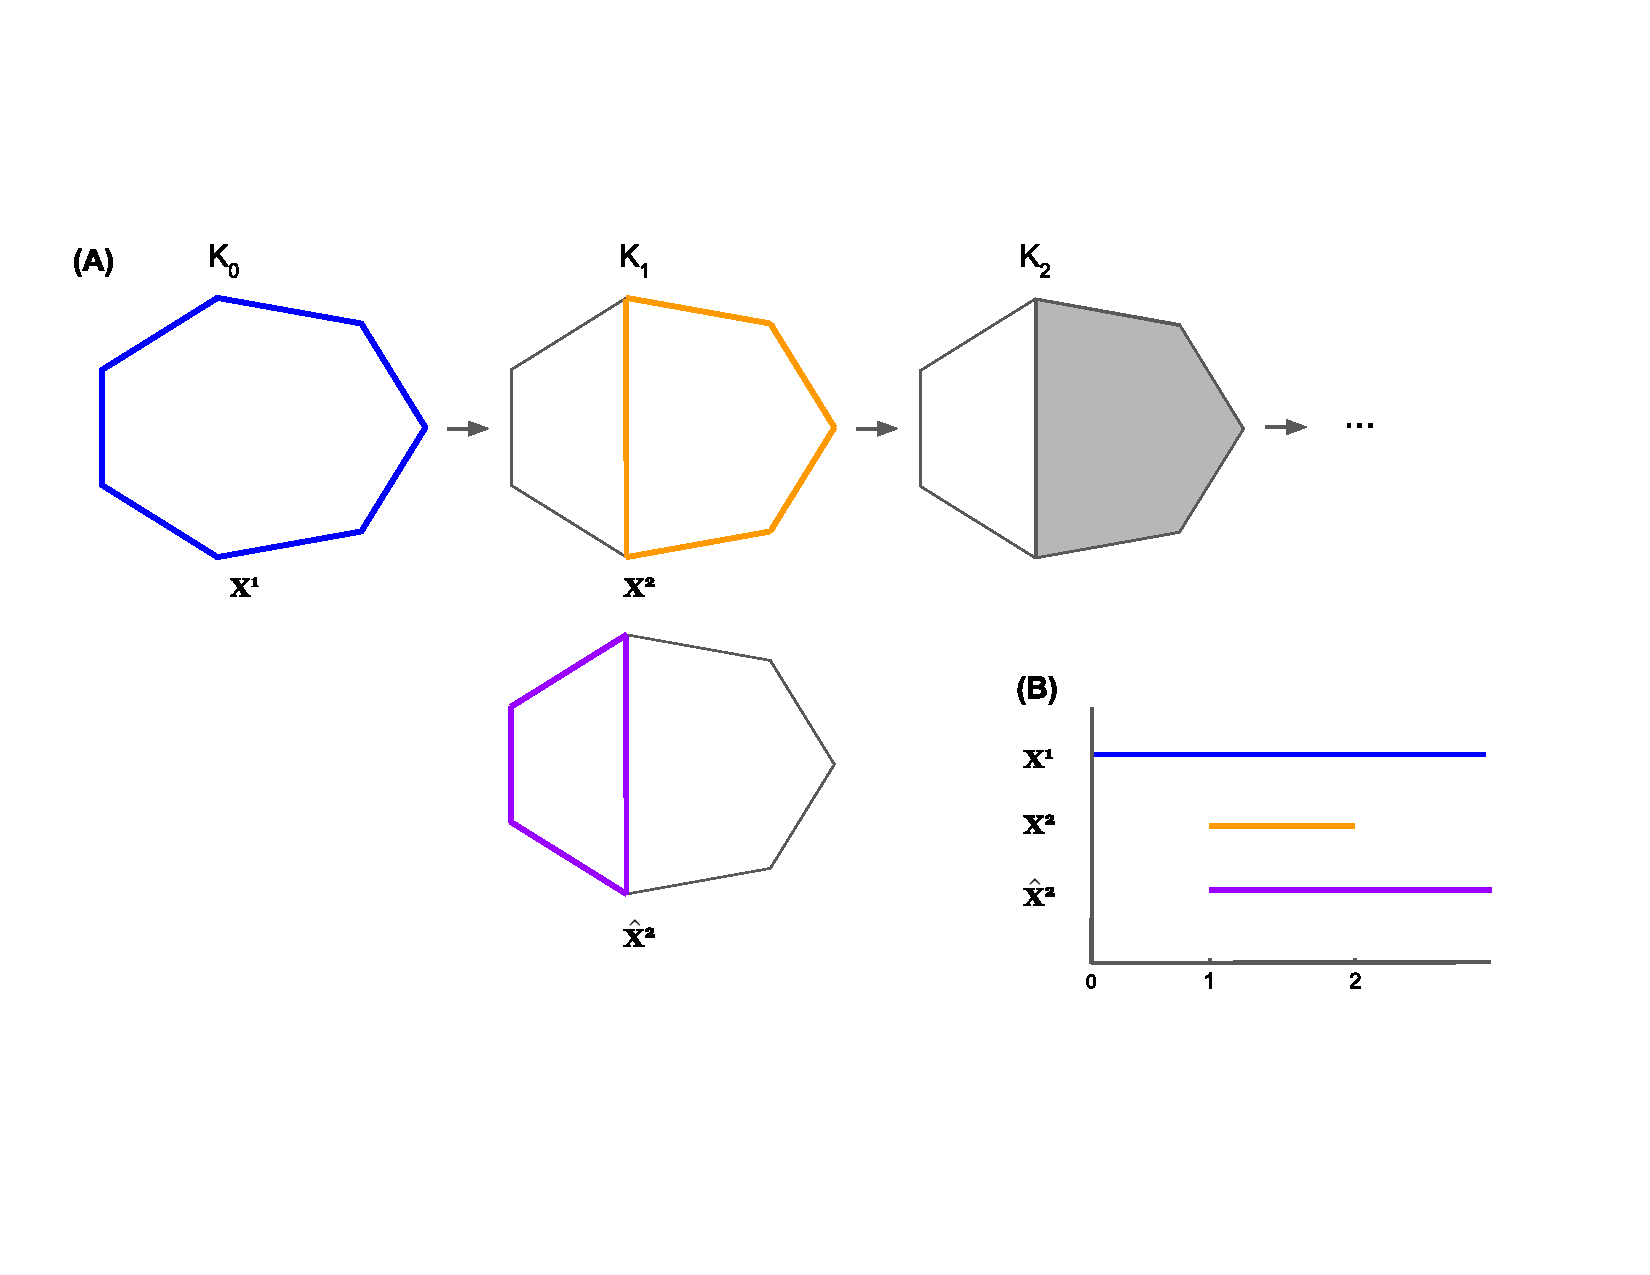
\includegraphics[width=1\textwidth]{figures/gregExample.pdf}% This is a *.eps file
\end{center}
\caption{An example where the optimal cycles obtained from \pr \eqref{eq:escolarargmin} do not form a persistent homological cycle basis. The thickened colored cycles in Subfigure (\textbf{A}) represent a cycle representative for the hole it encloses, and the bar with the corresponding color in Subfigure (\textbf{B}) records the lifespan of the cycle. In Subfigure (\textbf{A}), we see $\persinterval(\optimalrep^1) = [0,\infty), \persinterval(\optimalrep^2) = [1,2).$ Then, $\{\optimalrep^1, \optimalrep^2\}$ forms a basis for the persistent homological cycles. The cycle representative $\hat \optimalrep^2$ is an optimal cycle representative obtained by solving \pr (\ref{eq:filteredminimalbasis}) for the filtered simplicial complex $K_2$. However, $\persinterval(\hat \optimalrep_2) = [1, \infty)$, and thus  $\{\optimalrep^1, \hat \optimalrep^2\}$ is no longer a persistent homological cycle basis.} \label{fig:example-persBasis}
\end{figure}
